\documentclass[red]{TBUJournal}

%===----------------- CÁC GÓI LỆNH -------------------====
\usepackage{algorithm2e}
\usepackage{booktabs}
\usepackage{lineno}
\usepackage{tocloft,calc}
\usepackage{makeidx}

\newcommand{\scalefigure}{0.20}
\newcommand{\nothanks}{\protect\stepcounter{footnote}}

%===-------------- Title of the paper --------------------====
\title{TITLE OF THE PAPER IN ENGLISH. BE CONCISE, SPECIFIC AND RELEVANT. CAPITAL, BOLD, TIMES NEW ROMAN, SIZE 12}
\author[1]{Full name of author 1\thanks{Corresponding author: abc@xyz.com}}
\author[1]{Full name of author 2}
\author[2]{Full name of author 3}
%\author[1]{Full name of author 4}
\affil[1]{Affiliation for author 1}
\affil[2]{Affiliation for author 2}


\begin{document}
\pagestyle{tbuPageStyle}

\maketitle

%===------------------- ARTICLE INFO - KEYWORDS -----------------------====
\hrule
{\vskip 5pt}   
\noindent
\begin{minipage}[t]{0.39\textwidth} 
	\centerline{\fontsize{10}{10}\selectfont \textbf{ARTICLE INFO}}
	{\vskip 5pt}  
	\hrule
	{\vskip 6pt}  
	\begin{tabular}{rl}	
		\vspace{3pt}
		{\fontsize{9}{9}\selectfont \textbf{Received:}}	& {\fontsize{9}{9}\selectfont 26/10/2023}\\
		\vspace{3pt}
		{\fontsize{9}{9}\selectfont \textbf{Revised:}} & {\fontsize{9}{9}\selectfont 27/10/2023}\\
		\vspace{3pt}
		{\fontsize{9}{9}\selectfont \textbf{Published:}} & {\fontsize{9}{9}\selectfont 28/10/2023}\\	
	\end{tabular}
	\centerline{\fontsize{10}{10}\selectfont \textbf{KEYWORDS}}
	{\vskip 6pt}  
	\hrule
	{\vskip 3pt}  
	\keywords{Keyword 1, Keyword 2, Keyword 3, Keyword 4, Keyword 5} 
\end{minipage}
\hspace{8pt}%
\begin{minipage}[t]{0.6\textwidth}
	\centerline{\fontsize{10}{10} \textbf{ABSTRACT}}
	\noindent
	\begin{abstract}
		Trình bày tóm tắt bằng tiếng Anh. Nội dung khớp với tóm tắt tiếng Việt.		
	\end{abstract}
\end{minipage}

\begin{center}
	\fontsize{12}{14}\selectfont
	\textbf{TÊN BÀI BÁO BẰNG TIẾNG VIỆT. CẦN NGẮN GỌN, CHÍNH XÁC VÀ RIÊNG BIỆT. FONT TIME NEW ROMAN CỠ 12, IN ĐẬM}
\end{center}

\begin{flushleft}
	\textbf{\fontsize{10}{10}\selectfont Tên tác giả  1$^{*1}$, Tên tác giả 2$^1$, Tên tác giả  3$^2$}\\
	\textit{\fontsize{9}{9}\selectfont $^1$Đơn vị công tác của tác giả 1, 2, 4\\ $^2$Đơn vị công tác của tác giả 2}
\end{flushleft}
\vspace{6pt}

%===------------------- THÔNG TIN BÀI BÁO - TÓM TẮT -----------------------====
\hrule
{\vskip 1pt}   
\noindent
\begin{minipage}[t]{0.39\textwidth} 
\centerline{\fontsize{10}{10}\selectfont \textbf{THÔNG TIN BÀI BÁO}}
{\vskip 5pt}  
\hrule
{\vskip 3pt}  
	\begin{tabular}{rl}	
	\vspace{3pt}
	\textbf{\fontsize{9}{9}\selectfont Ngày nhận bài:}	& {\fontsize{9}{9}\selectfont 26/10/2023}\\
	\vspace{3pt}	
	\textbf{\fontsize{9}{9}\selectfont Ngày hoàn thiện:} & {\fontsize{9}{9}\selectfont 27/10/2023}\\
	\vspace{3pt}
	\textbf{\fontsize{9}{9}\selectfont Ngày đăng:}	& {\fontsize{9}{9}\selectfont 28/10/2023}\\	
	\end{tabular}
\centerline{\fontsize{10}{10}\selectfont \textbf{TỪ KHÓA}}
{\vskip 3pt}  
\hrule
{\vskip 3pt}  
\keywords{Từ khoá 1, Từ khoá 2, Từ khoá 3, Từ khoá 4, Từ khoá 5} 
\end{minipage}
\hspace{8pt}%
\begin{minipage}[t]{0.6\textwidth}
	\centerline{\fontsize{10}{10}\selectfont \textbf{TÓM TẮT}}
	\noindent
	\begin{abstract}
		Phần tóm tắt trình bày thành một đoạn văn, độ dài nằm trong khoảng 150-200 từ, không viết tắt, không chèn chú thích và tham chiếu tài liệu tham khảo (Nếu cần trích dẫn nguồn, ghi tên tác giả và năm ở trong ngoặc đơn). Nội dung tóm tắt cần bao gồm bốn ý sau: 1) Câu hỏi và mục đích của nghiên cứu. 2) Phương pháp nghiên cứu. Cần mô tả cách thức giải quyết vấn đề (phát triển lý thuyết/ phương pháp thu thập, xử lý dữ liệu…); 3)	Kết quả. Tóm tắt những kết quả chính của nghiên cứu, kể cả những số liệu có thể lấy làm điểm thiết yếu của nghiên cứu. 4) Kết luận. Một hoặc 2 câu văn kết luận và ý nghĩa của kết quả nghiên cứu. 
		Nội dung tóm tắt cần cung cấp thông tin một cách ngắn gọn, nhưng có dữ liệu minh chứng và đi thẳng vào vấn đề. 
	
		Lưu ý: hạn chế gõ công thức được định dạng trong tóm tắt, sẽ không hiển thị đúng trên các trang web.		
	\end{abstract}
\end{minipage}

\fontsize{11}{11}\selectfont

%===------------------ Introduction ---------------------====
\section{Maximal k-cliques}
\label{sec:introduction}



\subsection{An algorithm to discover the k-clique cover in networks~\cite{cavique2009algorithm}}


Khác với các hướng tiếp cận trước đó như [cite: 15] (dựa trên lý thuyết tập hợp) hay [cite: 16] (dựa trên cây tìm kiếm đệ quy), nghiên cứu [cite: 17] đề xuất một mô hình hai giai đoạn nhằm giải quyết bài toán bao phủ k-clique theo hướng toàn cục. Thay vì thực hiện các phép chỉnh sửa trực tiếp trên đồ thị, toàn bộ cấu trúc mạng được ánh xạ sang một biểu diễn ma trận phủ, qua đó ``làm phẳng'' độ phức tạp của bài toán đồ thị.

\subsubsection{Ý tưởng thuật toán}

Thuật toán đề xuất được chia thành hai pha độc lập nhưng liên kết chặt chẽ:
\begin{itemize}
	\item Pha 1: Tìm kiếm cụm bằng Meta-heuristic (Tabu Search). Không gian nghiệm được xây dựng thông qua các cấu trúc lân cận $N(S)$, với $S$ là tập đỉnh hiện tại. Ba toán tử chuyển trạng thái được định nghĩa.
	\begin{itemize}
		\item Thêm đỉnh: $N^+(S)={S'=S \cup \{v_i\}}$, với điều kiện vẫn bảo toàn tính chất k-clique.
		\item Xóa đỉnh: $N^-(S)={S'=S \backslash \{v_i\}}$.
		\item Hoán đổi: $N^0(S)={S'=S \cup \{v_i\} \backslash \{v_i\}}$.
	\end{itemize}
	Thông qua các toán tử này, thuật toán Tabu Search khám phá không gian nghiệm và thu thập tập các k-clique cực đại tiềm năng.
	
	\item Pha 2: Biểu diễn bài toán dưới dạng ma trận Set Covering. Sau khi hoàn tất pha tìm kiếm cụm, đồ thị ban đầu không còn được sử dụng. Thay vào đó, bài toán được chuyển sang một ma trận nhị phân $M[i,j]$ trong đó: Dòng  $i \in V$: đại diện cho các đỉnh cần được bao phủ; Cột $j \in C$: đại diện cho các cụm k-clique thu được từ pha 1; Biến quyết định $x_j \ in \{0,1\}$: xác định việc chọn cụm $j$.
	
	
\end{itemize}



















%
%Tài liệu này là bản mẫu về định dạng cho các bài báo in trên Tạp chí Khoa học và Công nghệ - Đại học Tây Bắc. Các yêu cầu cụ thể về định dạng, cấu trúc bài báo cũng được trình bày trong từng phần. 
%
%\textbf{Nếu bản thảo được soạn thảo bằng LaTex}, tác giả cần định dạng trang PDF xuất ra theo các quy định dưới đây. Bài báo phải được trình bày trên khổ A4 theo chiều dọc, với các thông số PageSetup cụ thể như sau: Top: 2 cm, Bottom: 2 cm, Left: 3,0 cm, Right: 2 cm, Header: 2,85cm, Footer: 2,85cm. Nội dung bài báo gõ bằng font chữ Times New Roman, cỡ 11, không dãn hay co cỡ chữ; chế độ dãn dòng: Single, khoảng trống dòng: before: 0, after: 0; căn lề justified. Khoảng thụt đầu dòng của đoạn văn là 0,5 cm. Tiêu đề các phần không thụt đầu dòng. Khoảng trống dòng của tiêu đề: before 6, after 6. Hình 1 mô tả thông số định dạng dãn dòng cho văn bản nội dung bài báo và thông số cho các tiêu đề.
%
%
%\setlength{\intextsep}{0pt}
%\renewcommand{\scalefigure}{0.73}
%\noindent
%\begin{figure}[h!]
%	\centering
%	\begin{subfigure}{.48\linewidth}
%		\centering
%		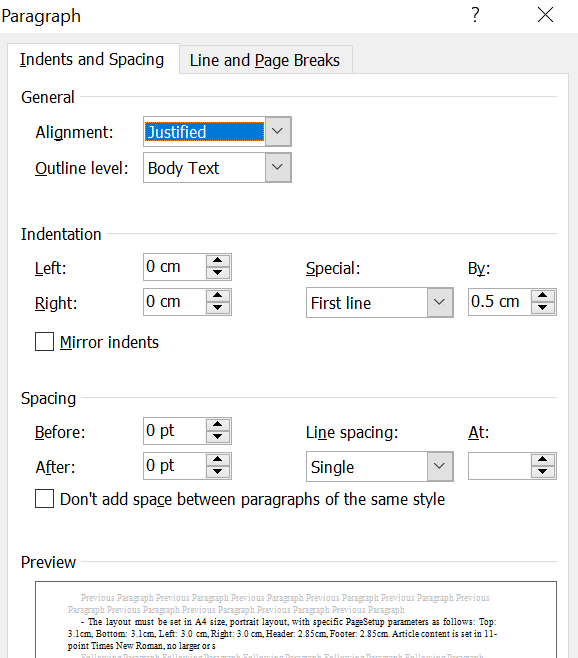
\includegraphics[scale=\scalefigure]{Pictures/pic1a.png}
%		\caption{}
%		\label{fig:format_a}
%	\end{subfigure}   
%	\begin{subfigure}{.48\linewidth}
%		\centering
%		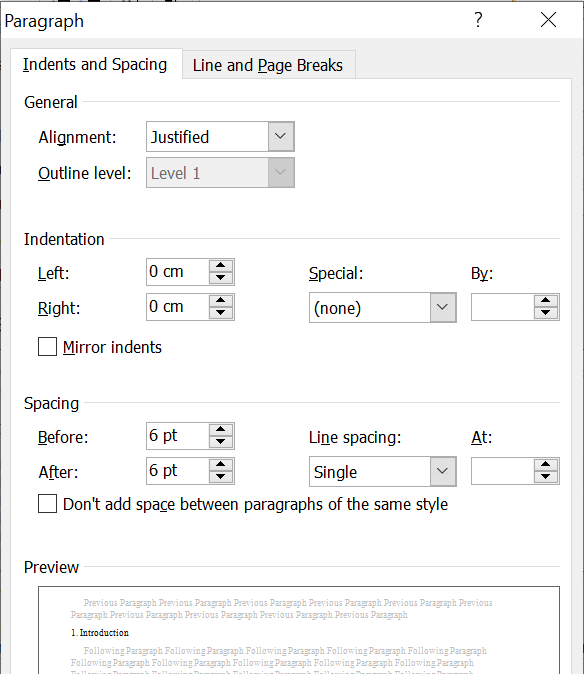
\includegraphics[scale=\scalefigure]{Pictures/pic1b.png}
%		\caption{}
%		\label{fig:format_b}
%	\end{subfigure}
%	\caption{Thông số định dạng cho (a): văn bản nội dung, (b): tiêu đề các phần}
%	\label{fig:format}
%\end{figure}
%
%Dung lượng mỗi bài báo không quá tám (08) trang, trừ những bài báo tổng quan (Review) – dung lượng từng bài dạng này do Ban biên tập xem xét cụ thể.
%
%Với bài báo soạn thảo bằng MS. Word, tác giả có thể không cần định dạng theo mẫu này. Tòa soạn sẽ dàn trang nếu bài báo được chấp nhận đăng.
%
%Bài báo cần được viết theo cấu trúc IMRAD (Introduction – Methods/Materials – Results – And Discussion. Cấu trúc IMRAD là một cấu trúc đặc thù, phổ biến trong cộng đồng khoa học quốc tế. Tiêu đề các phần chính của bài báo (Tiêu đề cấp 1) dùng chữ in đậm, cùng cỡ chữ (11 pt) với cỡ chữ của nội dung bài báo. Tiêu đề cấp 2 dùng chữ in đậm, nghiêng. Tiêu đề cấp 3 dùng chữ in nghiêng. Ví dụ định dạng tiêu đề các cấp như sau:\\
%\textbf{1. Tiêu đề cấp 1}\\
%\textbf{\textit{1.1. Tiêu đề cấp 2}}\\
%\textit{1.1.1. Tiêu đề cấp 3}\\
%\textit{1.1.2. Tiêu đề cấp 3}\\
%\textbf{\textit{1.2. Tiêu đề cấp 2}}\\
%...\\
%\textbf{\textit{2. Tiêu đề cấp 1}}
%
%\textbf{Lưu ý:} Không sử dụng chế độ đánh số tự động. Không dùng tiêu đề quá cấp 3.
%
%Nội dung phần Giới thiệu cần cung cấp những thông tin sau: vấn đề nghiên cứu đặt ra là gì, đã có những công trình nghiên cứu nào thực hiện để giải quyết vấn đề, và khoảng trống của tri thức cần được bổ sung là gì, từ đó chỉ ra mục đích nghiên cứu. Do dung lượng bài báo không quá 8 trang, nên không bố trí phần “tổng quan tài liệu” riêng.
%
%Nên cấu trúc phần Giới thiệu như sau:
%
%Trước hết, cung cấp thông tin ngắn gọn về hoàn cảnh đặt ra vấn đề cần nghiên cứu. Nếu cần, sử dụng 1-2 câu văn tóm tắt kiến thức cơ bản có liên quan trực tiếp đến vấn đề nghiên cứu. Phát biểu vấn đề nghiên cứu một cách cụ thể, súc tích. Thứ hai, thông qua việc tóm tắt các kết quả nghiên cứu liên quan đã được công bố gần nhất, chỉ ra khoảng trống về kiến thức cần bổ sung để hoàn thiện lời giải cho vấn đề nghiên cứu. Các kết quả nghiên cứu liên quan đến vấn đề nghiên cứu nhất thiết phải kèm theo trích dẫn, tham chiếu đến tài liệu tham khảo. Số lượng trích dẫn trong phần giới thiệu tối thiểu bằng số trang của bài báo, trong đó có ít nhất 5 bài báo khoa học công bố gần nhất. Nếu quá ít trích dẫn, có thể được hiểu rằng hoặc vấn đề ít quan trọng nên ít người quan tâm, hoặc tác giả không chịu tìm hiểu vấn đề đã được quan tâm giải quyết thế nào, khoảng trống kiến thức khoa học cần bổ sung là gì. Nên trích dẫn các công bố khoa học trên các tạp chí uy tín. Riêng bài báo tổng quan, cần đảm bảo có ít nhất 10 tài liệu tham khảo là các bài báo khoa học. Trong lộ trình nâng cao chất lượng Tạp chí Khoa học Đại học Tây Bắc theo chuẩn quốc tế, tác giả cần ưu tiên trích dẫn các bài báo đã đăng trên các tạp chí trong danh mục ISI, Scopus, ACI. Thông tin dùng cho trích dẫn (Metadata – siêu dữ liệu – dữ liệu mô tả) của mỗi bài báo đã đăng trên Tạp chí Khoa học Đại học Tây Bắc có thể dễ dàng download từ trang web của Tạp chí. Nếu trích dẫn từ các tạp chí trong nước, cần chỉ rõ tên đơn vị chủ quản của Tạp chí để người đọc tìm được nguồn tài liệu khi cần. 
%
%Khi trích dẫn, không nên tham chiếu đến sách giáo khoa, giáo trình, luận văn cao học. Chỉ khi nhất thiết phải sử dụng kiến thức/ công thức cơ sở trong các sách giáo trình để phát triển lý thuyết hay áp dụng cho tính toán thiết kế trong nghiên cứu thì mới trích dẫn từ các tài liệu tham khảo là sách giáo trình. 
%
%Tiếp theo, nên mô tả ngắn gọn cách thức và kết quả thu được để giải quyết vấn đề đã nêu. 
%Cuối phần Giới thiệu, nên mô tả tóm tắt nội dung các phần tiếp theo của bài báo để người đọc tiện theo dõi.


%===----------------- Proposed algorithm ----------------====
\section{Lớp bài toán phủ đồ thị bởi s-club}
\label{sec:proposedAlgorithm}
%===----------------- subsection Covering a Graph with Clubs ----------------====
\subsection{Phát biểu bài toán <<<< THAY BẰNG PHÁT BIỂU TỔNG QUÁT HOẶC PHÁT BIỂU RIÊNG TỪNG BÀI}
Cho đơn đồ thị vô hướng $G=(V, E)$ với tập đỉnh $V$, tập cạnh $E$. Mỗi tập đỉnh $S \subseteq V$, ký hiệu $G[S]$ là đồ thị con cảm sinh bởi tập $S$. Cho hai đỉnh $u,v \in V$, khoảng cách giữa $u$ và $v$ trên đồ thị $G$, ký hiệu bởi $d_G (u,v)$ là số cạnh trên đường ngắn nhất nối từ $u$ tới $v$.

Định nghĩa 1 (đường kính của đồ thị).

Đường kính của đơn đồ thị vô hướng $G=(V, E)$ (ký hiệu diam(G)) là khoảng cách lớn nhất giữa hai đỉnh bất kỳ của tập $V$.

Định nghĩa 2 (s-club)

Cho đơn đồ thị vô hướng $G=(V, E)$ và tập con $U \subseteq V$, đồ thị con $G[U]$ là một s-club nếu đường kính của $G[U]$ lớn nhất là $s (diam(G[U]) \leq s)$.

Định nghĩa 3 (bài toán Minimum s-club cover)

Cho đơn đồ thị vô hướng $G=(V, E)$ và một số nguyên $s \geq 2$, hãy tìm tập $C={C_1,C_2,\ldots, C_h}$ nhỏ nhất sao cho với mỗi $i (1 \leq i \leq h)$ và tập $C_i \subseteq V$ thì $G[C_i]$ là một s-club và với mỗi đỉnh $v\in V$, tồn tại một tập $Cj (1 \leq j \leq h)$ sao cho $v \in C_j$.

Hình~\ref{fig:sClub_Definition} minh họa một lời giải của bài toán Minimum 2-club cover đối với đồ thị có 9 đỉnh gồm hai club: $C_1 = \{1, 2, 3, 4, 5\}$, $C_2 = \{5, 6, 7, 8, 9\}$.


\setlength{\intextsep}{0pt}
\renewcommand{\scalefigure}{0.6}
\noindent
\begin{figure}[h!]
	\centering
	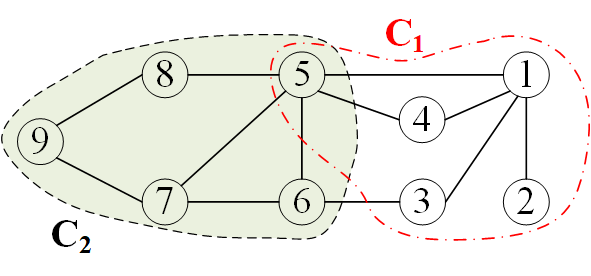
\includegraphics[scale=\scalefigure]{Pictures/sClub_cover/Definition_1.png}
%	\begin{subfigure}{.48\linewidth}
%		\centering
%		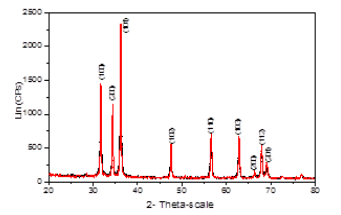
\includegraphics[scale=\scalefigure]{Pictures/pic2a.png}
%		\caption{}
%		\label{fig:giando_a}
%	\end{subfigure}   
%	\begin{subfigure}{.48\linewidth}
%		\centering
%		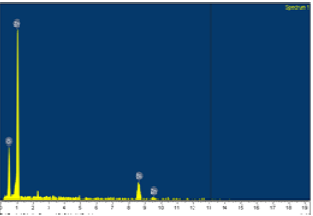
\includegraphics[scale=\scalefigure]{Pictures/pic2b.png}
%		\caption{}
%		\label{fig:giando_b}
%	\end{subfigure}
	\caption{Lời giải bài toán Minimum s-club cover}
	\label{fig:sClub_Definition}
\end{figure}


%===----------------- subsection Covering a Graph with Clubs ----------------====
\subsection{Covering a Graph with Clubs~\cite{dondi2019covering}}
Nghiên cứu [cite: 19] tiếp cận bài toán phân cụm theo hướng bảo toàn cấu trúc đồ thị, thông qua mô hình bao phủ toàn cục thay vì các thao tác chỉnh sửa mang tính phá hủy như xóa đỉnh [cite: 15], [cite: 16] hay xóa cạnh [cite: 18]. Mục tiêu của bài toán là tìm một tập tối thiểu các cụm s-club sao cho mọi đỉnh trong đồ thị đều được bao phủ.

Điểm cốt lõi trong mô hình hóa nằm ở việc cho phép các cụm chồng lấp lên nhau. Một đỉnh có thể đồng thời thuộc nhiều cụm khác nhau, phản ánh đúng đặc tính của các mạng thực tế, nơi một thực thể có thể tham gia vào nhiều cộng đồng.

Mặc dù trong nghiên cứu~\cite{dondi2019covering}, các tác giả đã đề xuất thuật toán gần đúng Club-Cover-Approx (ký hiệu CCA) tìm được lời giải bài toán Minimum 2-club cover với hệ số $2|V|^{1/2}\log^{3/2}|V|$, trong đó $V$ là tập đỉnh của đồ thị, $|V|$ là số đỉnh của tập $V$. Tại mỗi bước, thuật toán CCA sẽ tìm một 2-club là tập lớn nhất các đỉnh được chọn. Mặc dù thuật toán CCA có ưu điểm về thời gian thực hiện và đơn giản về ý tưởng lẫn cài đặt thuật toán, tuy nhiên do dựa trên chiến lược tham lam và chất lượng lời giải phụ thuộc nhiều vào bậc của các đỉnh của đồ thị đầu vào nên chất lượng lời giải mà thuật toán chưa thực sự tốt. Bên cạnh đó, thuật toán CCA chỉ giải bài toán Minimum 2-club cover, không áp dụng để giải được các bài toán Minimum s-club cover với $s > 2$.

>>>>>>>>>>>>>>>>>> THÊM MÔ TẢ VỀ CÁC BƯỚC THUẬT TOÁN


Thuật toán này được thiết kế để tìm một tập hợp các $2$-club bao phủ toàn bộ các đỉnh của đồ thị $G = (V, E)$ với số lượng club ít nhất có thể.


Thuật toán hoạt động thông qua một vòng lặp liên tục cho đến khi tất cả các đỉnh đều được bao phủ:

\begin{itemize}
    \item {Bước 1: Khởi tạo (Initialization):}
    
    Thiết lập tập hợp các đỉnh chưa được bao phủ:
    \[
    V' = V
    \]
    
    Khởi tạo tập lời giải rỗng:
    \[
    \mathcal{S} = \emptyset
    \]

    \item {Bước 2: Lựa chọn tham lam (Greedy Choice):}
    
    Trong mỗi vòng lặp, thuật toán tìm kiếm một đỉnh $v \in V$ sao cho kích thước của tập giao giữa vùng lân cận đóng của nó và tập đỉnh chưa bao phủ là lớn nhất:
    \[
    |N[v] \cap V'| \rightarrow \max
    \]
    
    Ở đây, $N[v]$ bao gồm đỉnh $v$ và tất cả các đỉnh kề trực tiếp với nó.

    \item {Bước 3: Cập nhật lời giải (Update):}
    
    Thêm tập hợp các đỉnh $N[v]$ vào tập lời giải:
    \[
    \mathcal{S} = \mathcal{S} \cup \{N[v]\}
    \]
    
    Loại bỏ các đỉnh đã được bao phủ bởi $N[v]$ ra khỏi tập:
    \[
    V' = V' \setminus N[v]
    \]

    \item {Bước 4: Điều kiện dừng (Termination):}
    
    Nếu $V' \neq \emptyset$, quay lại Bước 2.
    
    Nếu $V' = \emptyset$, trả về tập $\mathcal{S}$ là tập hợp các $2$-club bao phủ đồ thị.
\end{itemize}





\subsubsection{Ưu điểm}
Phương pháp thể hiện khả năng mô hình hóa tốt các đặc tính của mạng thực tế thông qua việc cho phép chồng lấp giữa các cụm. Ràng buộc bao phủ với điều kiện lớn hơn hoặc bằng một đóng vai trò như cơ chế logic trung tâm để biểu diễn các đỉnh cầu nối mà không cần thực hiện các thao tác chỉnh sửa cấu trúc đồ thị.

Ngoài ra, việc kết hợp chiến lược tham lam với bước cắt tỉa giúp cải thiện hiệu quả sử dụng bộ nhớ. Ngay cả khi nghiệm ban đầu chứa các cụm dư thừa, hệ thống vẫn có khả năng loại bỏ các phần tử không cần thiết để giảm kích thước lớp phủ cuối cùng.


\subsubsection{Nhược điểm}
Phương pháp phụ thuộc nhiều vào bước tạo các s-club cực đại. Tại bước này, số lượng s-club có thể tăng theo cấp số mũ khi đồ thị là đồ thị dày hoặc khi giá trị tham số s lớn.

Bên cạnh đó, việc sử dụng thuật toán tham lam có thể dẫn tới việc làm suy giảm chất lượng nghiệm. Chiến lược ưu tiên các s-club lớn trong giai đoạn đầu có thể dẫn đến việc bỏ sót các đỉnh ở lân cận, buộc phải chọn các s-club có số lượng đỉnh ít ở giai đoạn cuối. Hệ quả là số lược các s-club để phủ hết các đỉnh có thể lớn hơn đáng kể so với lời giải tối ưu.


%===----------------- subsection Covering a Graph with Clubs ----------------====
\subsection{Thuật toán gần đúng dựa trên phương thức khởi tạo lời giải nhiều lần giải bài toán minimum s-club cover~\cite{thanh2023}}

Trong nghiên cứu~\cite{thanh2023}, các tác giả đã đề xuất thuật toán dựa trên phương pháp khởi tạo lời giải nhiều lần sử dụng chiến lược tham lam để tìm club tốt nhất tại mỗi bước. Nghiên cứu cũng đề xuất phương pháp tạo lân cận của lời giải đang xét được tạo bằng cách di chuyển một đỉnh sang một club khác. Để so sánh các cá thể, đề xuất định nghĩa hàm đánh giá cá thể khác hàm mục tiêu của bài toán Minimum s-club cover để so sánh các lân cận của lời giải đang xét dựa trên tổng số club của lời giải và tỉ số giữa số đỉnh của club có số lượng đỉnh nhỏ nhất chia cho số đỉnh của đồ thị đầu vào. Thuật toán được đề xuất gồm các bước chính sau:
\begin{itemize}
	\item Bước 1: Sử dụng thuật toán CCA để khởi tạo lời giải của bài toán Minimum s-club cover, lời giải này được đặt là lời giải hiện thời.
	\item Bước 2: Lặp lại các bước sau:
	\begin{itemize}
		\item Bước 2.1. Tạo danh sách các lân cận tốt nhất của lời giải hiện thời (mô tả chi tiết trong phần 2.3). Nếu không tìm được lân cận nào tốt hơn lời giải hiện thời thì thoát khỏi vòng lặp.
		
		\item Bước 2.2. Chọn ngẫu nhiên một trong các lời giải từ Bước 2.1 đặt làm lời giải hiện thời.
		
		\item Bước 2.3. Nếu sau một số lần xác định trước lời giải tốt nhất tìm được không được cải thiện thì thoát khỏi vòng lặp.
	\end{itemize}
\end{itemize}

>>>> THÊM HẠN CHẾ CỦA ĐỀ XUẤT


\subsubsection{Ưu điểm}

    Thuật toán giải quyết được bài toán Minimum $s$-club cover cho trường hợp tổng quát $s \ge 2$, khắc phục trực tiếp hạn chế của thuật toán CCA tiền nhiệm vốn chỉ áp dụng được cho $s=2$.
    
    Bằng cách áp dụng phương thức đa khởi tạo (MSM) kết hợp với chiến lược tham lam trong việc tạo lân cận, thuật toán I-MSM cho kết quả tốt hơn CCA trên $1/3$ bộ dữ liệu thử nghiệm từ thư viện DIMACS và bằng nhau trên $2/3$ bộ còn lại.
    
    Tối ưu hóa hàm đánh giá: Nghiên cứu đề xuất hàm đánh giá mới:
    \[
    f(sol) = num\_club + \frac{min\_vertex}{|V|}
    \]
    Công thức này giúp thuật toán ưu tiên các lời giải có club nhỏ chứa ít đỉnh hơn, từ đó tăng khả năng chuyển các đỉnh này sang club khác để nhanh chóng giảm số lượng club.

\subsubsection{Nhược điểm}

    Thuật toán vẫn phải gọi CCA để khởi tạo lời giải hiện thời. Do CCA là thuật toán tham lam, chất lượng lời giải gốc chưa thực sự tốt và vẫn bị phụ thuộc vào đồ thị đầu vào.
    
    Khi xét club để chuyển đỉnh, thuật toán đánh giá chi phí bằng chính số lượng đỉnh của club đó ($cost_{cl} = |cl|$). Cơ chế này dẫn tới việc luôn ưu tiên lựa chọn các club đã có sẵn kích thước lớn, dễ làm giảm tính đa dạng trong không gian tìm kiếm lân cận.
    
    Việc sinh lân cận yêu cầu tính toán lại đường kính của đồ thị con cảm sinh liên tục để kiểm tra điều kiện $radius < s$. Với cấu hình thử nghiệm lên tới $50{,}000$ lần đánh giá, thuật toán tiêu tốn nhiều tài nguyên tính toán.
    
    I-MSM chưa đảm bảo nghiệm tối ưu toàn cục. Hướng phát triển tiếp theo bắt buộc phải kết hợp với các thuật toán dựa trên quần thể để cải thiện triệt để chất lượng lời giải.








%===----------------- subsection Covering a Graph with Clubs ----------------====
\subsection{Áp dụng thuật toán di truyền nhóm giải bài toán minimum s-club cover~\cite{}}

Thuật toán di truyền nhóm (Grouping Genetic Algorithm - GGA) được đề xuất áp dụng vào giải bài toán Minimum s-club cover problem. Nghiên cứu tập trung vào các xây dựng toán tử tiến hoá và phương pháp đánh giá lời giải bài toán Minimum s-club cover.

Nghiên cứu sử dụng toán tử lai ghép gồm 6 bước được cải tiến từ toán tử lai ghép Falkenauer~\cite{falkenauer1994new} bằng cách sử dụng phương pháp chọn ngẫu nhiên các club để gán cho các gen chưa có giá trị. Toán tử lai ghép được đề xuất đảm bảo các cá thể con được tạo ra từ cá thể cha mẹ hợp lên luôn hợp lệ. Toán tử đột biến được các tác giả đề xuất dựa trên việc sử dụng ngẫu nhiên ba toán tử đột biến: Tách club, kết hợp hai club và chuyển club với tỉ lệ tương đương nhau. Các cá thể trong nghiên cứu được đánh giá thông qua đường kính của đồ thị con cảm sinh có đường kính lớn nhất.

>>>> THÊM MỔ TẢ VỀ LAI GHÉP, ĐỘT BIẾN, ĐÁNH GIÁ hoặc ví dụ minh hoạ.

>>>> THÊM HẠN CHẾ, ƯU ĐIỂM CỦA ĐỀ XUẤT




%===----------------- subsection Covering a Graph with Clubs ----------------====
\subsection{A Hybrid Multifactorial Evolutionary Algorithm for the Minimum s-Club Cover Problem~\cite{thanh2024hybrid}}

Nghiên cứu đề xuất kết hợp thuật toán tìm kiếm cục bộ vào thuật toán tiến hoá đa nhân tố. Tại mỗi thế hệ, thuật toán tìm kiếm cục bộ sẽ áp dụng đối với lời giải tốt nhất của mỗi tác vụ. Thuật toán tìm cục bộ sẽ chọn ngẫu nhiên một đỉnh của đồ thị và thử chuyển đỉnh được chọn tới club khác. Nếu chất lượng lời giải không được cải thiện sau khi chuyển đỉnh thì đỉnh sẽ được đưa về club trước khi thử chuyển.


>>>> THÊM MỔ TẢ VỀ LAI GHÉP, ĐỘT BIẾN, ĐÁNH GIÁ hoặc ví dụ minh hoạ.

>>> Có thể thêm lược đồ thuật toán

>>>> THÊM HẠN CHẾ, ƯU ĐIỂM CỦA ĐỀ XUẤT


%===----------------- subsection Covering a Graph with Clubs ----------------====
\subsection{Evolutionary multitasking algorithm based on a dynamic solution encoding strategy for the minimum s-club cover problem~\cite{thanh2025evolutionary}}

Các tác giả đề xuất thuật toán tiến hóa đa nhiệm giải bài toán minimum s-club cover. Trong đó, các tác giả tập trung vào xây dựng phương pháp biểu diễn lời giải của một bài toán minimum s-club cover và biểu diễn lời giải trong không gian biểu diễn chung khi dùng thuật toán tiến hóa đa nhiệm giải nhiều bài toán minimum s-club cover. Mỗi lời giải được biểu diễn bởi hai phần tách biệt: 
\begin{itemize}
	\item Phần thông tin về các club: xác định số lượng club và nhãn club sử dụng để mã hóa lời giải.
	
	\item Phần thông tin về các đỉnh: phần này có chiều dài bằng số lượng đỉnh của đồ thị đầu vào. Mỗi giá trị sẽ xác định club mà đỉnh tương ứng thuộc về.
\end{itemize}
Mỗi cá thể trong không gian biểu diễn chung cũng được mã hóa gồm hai phần như đối với cá thể, trong đó, phần mã hóa club lưu trữ số club lớn nhất của lời giải các bài toán; phần thông tinh các đỉnh lưu trữ đỉnh của bài toán đầu vào có số chiều lớn nhất.

Một trong những đóng góp chính của nghiên cứu là đề xuất phương pháp khởi tạo lời giải bản đầu sử dụng thuật toán tham lam ngẫu nhiên (ký hiệu: Meta-RaPS). Phương pháp sẽ lặp lại việc xác định các club có đường kính nhỏ hơn $s$ cho tới khi tất cả các đỉnh của đồ thị đầu vào được gán vào ít nhất một club. Để đảm bảo đường kính của club được tạo luôn nhỏ hơn $s$, phương pháp khởi tạo lời giải thực hiện $s-1$ lần việc thêm một đỉnh là lân cận của một trong các đỉnh đã được thêm vào club ở các bước trước đó.

Trong nghiên cứu, các tác giả cũng đề xuất toán tử lai ghép gồm 6 bước chính bắt đầu bằng việc chọn ngẫu nhiên các club và các đỉnh thuộc club từ một cá thể cha mẹ. Sau đó, các đỉnh được chọn sẽ được thay thế vào các đỉnh thuộc các club tương ứng trên cá thể mẹ còn lại. Nếu sau khi thay thế vẫn còn định chưa được sử dụng thì các đỉnh này sẽ được thêm vào club mới. Nhằm tăng độ đa dạng của quần thể, nghiên cứu đề xuất toán tử đột biến gồm hai giai đoạn: giai đoạn đầu sẽ chọn chọn ngẫu nhiên một club có ít nhất hai đỉnh; giải đoạn sau sẽ chuyển ngẫu nhiên một đỉnh trong club được chọn sang club khác. Toán tử đột biến mới được kết họp với hai toán tử đột biến khác với tỉ lệ gần tương đương nhau để tạo thành toán tử đột biến sử dụng trong thuật toán tiến hóa đa nhiệm.

>>> Chi tiết thêm về biểu diễn lời giải, hình ví dụ

>>> CHi tiết thêm về phương pháp khởi tạo lời giải

>>> Chi tiết về thuật toán đề xuất, vẽ sơ đồ.

>>>> THÊM HẠN CHẾ, ƯU ĐIỂM CỦA ĐỀ XUẤT


%===----------------- subsection Covering a Graph with Clubs ----------------====
\subsection{New Local Search Strategy for the Minimum s-Club Cover Problem~\cite{dinh2025new}}

Nghiên cứu trình bày kết hợp giữa thuật toán tiến hoá và thuật toán tìm kiếm cục bộ, trong đó tập trung vào đề xuất thuật toán tìm kiếm cục bộ dựa trên kết hợp chiến lược tham lam để xác định club và chiến lược vét cạn để chuyển một đỉnh lại club. Điểm khác biệt của thuật toán tìm kiếm cụ bộ được đề xuất là xử lý đối với club thay vì đối với đỉnh. Thuật toán thử xoá các đỉnh trên club có số đỉnh ít nhất hoặc club được chọn ngẫu nhiên từ tập các club có số lượng đỉnh nhiều hơn số club có ít đỉnh nhất một tỉ lệ cho trước. Với club được chọn, thuật toán sẽ thủ di chuyển các đỉnh có bậc 1 hoặc bậc 0 tới các club khác. Đỉnh sẽ chỉ được chuyển sang club khác nếu club sau khi thêm đỉnh được chuyển vào vẫn thoả mãn điều kiện của một s-Club.


>>>> CÓ THỂ THÊM MÔ TẢ VỀ THUẬT TOÁN DI TRUYỀN/TIẾN HOÁ: LAI GHÉP, ĐỘT BIẾN,...

>>>> THÊM HẠN CHẾ, ƯU ĐIỂM CỦA ĐỀ XUẤT


Nghiên cứu áp dụng phương pháp mã hóa trực tiếp từ đỉnh đến cụm (vertex-to-cluster encoding). 
Phương pháp này mang lại sự linh hoạt trong việc xử lý số lượng cụm biến đổi và giúp bảo tồn các cấu trúc có ý nghĩa trong suốt quá trình tiến hóa.

\begin{itemize}
    \item{Cấu trúc cá thể:} Mỗi nhiễm sắc thể (cá thể) được chia thành hai phân đoạn chính:
    \begin{itemize}
        \item {Phân đoạn câu lạc bộ (Club section):} Chứa thông tin về các nhãn của $s$-Club.
        
        \item{Phân đoạn đỉnh (Vertices section):} Xác định nhãn câu lạc bộ mà mỗi đỉnh được gán vào.
    \end{itemize}

    \item{Không gian tìm kiếm hợp nhất (Unified Search Space -- USS):} Chiều dài của mỗi phân đoạn trong một cá thể thuộc USS được thiết lập bằng với số chiều của nhiệm vụ lớn nhất (tức là nhiệm vụ có số đỉnh nhiều nhất).

    \item{Quy trình giải mã (Decoding):} Đối với một nhiệm vụ cụ thể có kích thước $m$, thuật toán giải mã bằng cách trích xuất $m$ gen đầu tiên từ phân đoạn đỉnh của cá thể trong USS. 
    Phân đoạn câu lạc bộ sau đó được tái thiết lập thông qua việc gán lại nhãn (relabeling) các giá trị gen, nhằm đảm bảo các nhãn câu lạc bộ được đánh số tuần tự và nhất quán.
\end{itemize}
>>>  hình ví dụ

Ví dụ cá thể trong không gian hợp nhất (USS)
Kích thước tối đa của USS: $D_{USS} = 10$
\begin{verbatim}
Phân đoạn Clubs   : | 1 | 2 | 3 |
Phân đoạn Vertices: | 1 | 1 | 1 | 1 | 3 | 2 | 2 | 3 | 2 | 2 |
                      ^   ^   ^   ^   ^   ^   ^   ^   ^   ^
Đỉnh tương ứng    :   1   2   3   4   5   6   7   8   9   10
\end{verbatim}
Giải mã cho nhiệm vụ có 8 đỉnh

Kích thước nhiệm vụ: $D_{t} = 8$

Trích xuất $8$ gen đầu tiên, loại bỏ $2$ gen cuối:

\begin{verbatim}
Phân đoạn Clubs   : | 1 | 2 | 3 |
Phân đoạn Vertices: | 1 | 1 | 1 | 1 | 3 | 2 | 2 | 3 |
\end{verbatim}

Kết quả:
\begin{itemize}
    \item Club 1 chứa các đỉnh: $\{1, 2, 3, 4\}$
    \item Club 2 chứa các đỉnh: $\{6, 7\}$
    \item Club 3 chứa các đỉnh: $\{5, 8\}$
\end{itemize}

Quá trình khởi tạo quần thể đóng vai trò nền tảng trong việc định hướng quỹ đạo tiến hóa của toàn bộ thuật toán.

\begin{itemize}
    \item {Khởi tạo ngẫu nhiên kết hợp tham lam:} Ban đầu, thuật toán sinh ra một quần thể $P(0)$ gồm các cá thể được khởi tạo ngẫu nhiên. Tuy nhiên, nhằm nâng cao chất lượng lời giải ngay từ thế hệ đầu tiên, một chiến lược tham lam (greedy strategy) được tích hợp vào quá trình khởi tạo. Cơ chế này giúp các cá thể ban đầu hình thành các cấu trúc mạng lưới tương đối phù hợp với các ràng buộc của mô hình $s$-Club, từ đó tạo tiền đề thuận lợi cho các bước tiến hóa tiếp theo.
    
    \item {Gán hệ số kỹ năng (Skill Factor):} Sau khi khởi tạo, mỗi cá thể trong quần thể $P(0)$ được đánh giá hiệu suất trên toàn bộ các nhiệm vụ. Dựa trên kết quả đánh giá này, mỗi cá thể được gán một hệ số kỹ năng, đại diện cho nhiệm vụ mà cá thể đó có khả năng giải quyết hiệu quả nhất. Thông tin này đóng vai trò quan trọng trong việc điều phối quá trình chuyển giao tri thức giữa các nhiệm vụ trong khuôn khổ tối ưu hóa đa nhiệm.
\end{itemize}
\setlength{\intextsep}{4pt}
\setlength{\textfloatsep}{6pt}
\setlength{\abovecaptionskip}{2pt}
\setlength{\belowcaptionskip}{2pt}

% caption nhỏ gọn
\captionsetup{
    font=small,
    labelfont=bf
}

\noindent
\begin{figure}[h!]
    \centering
    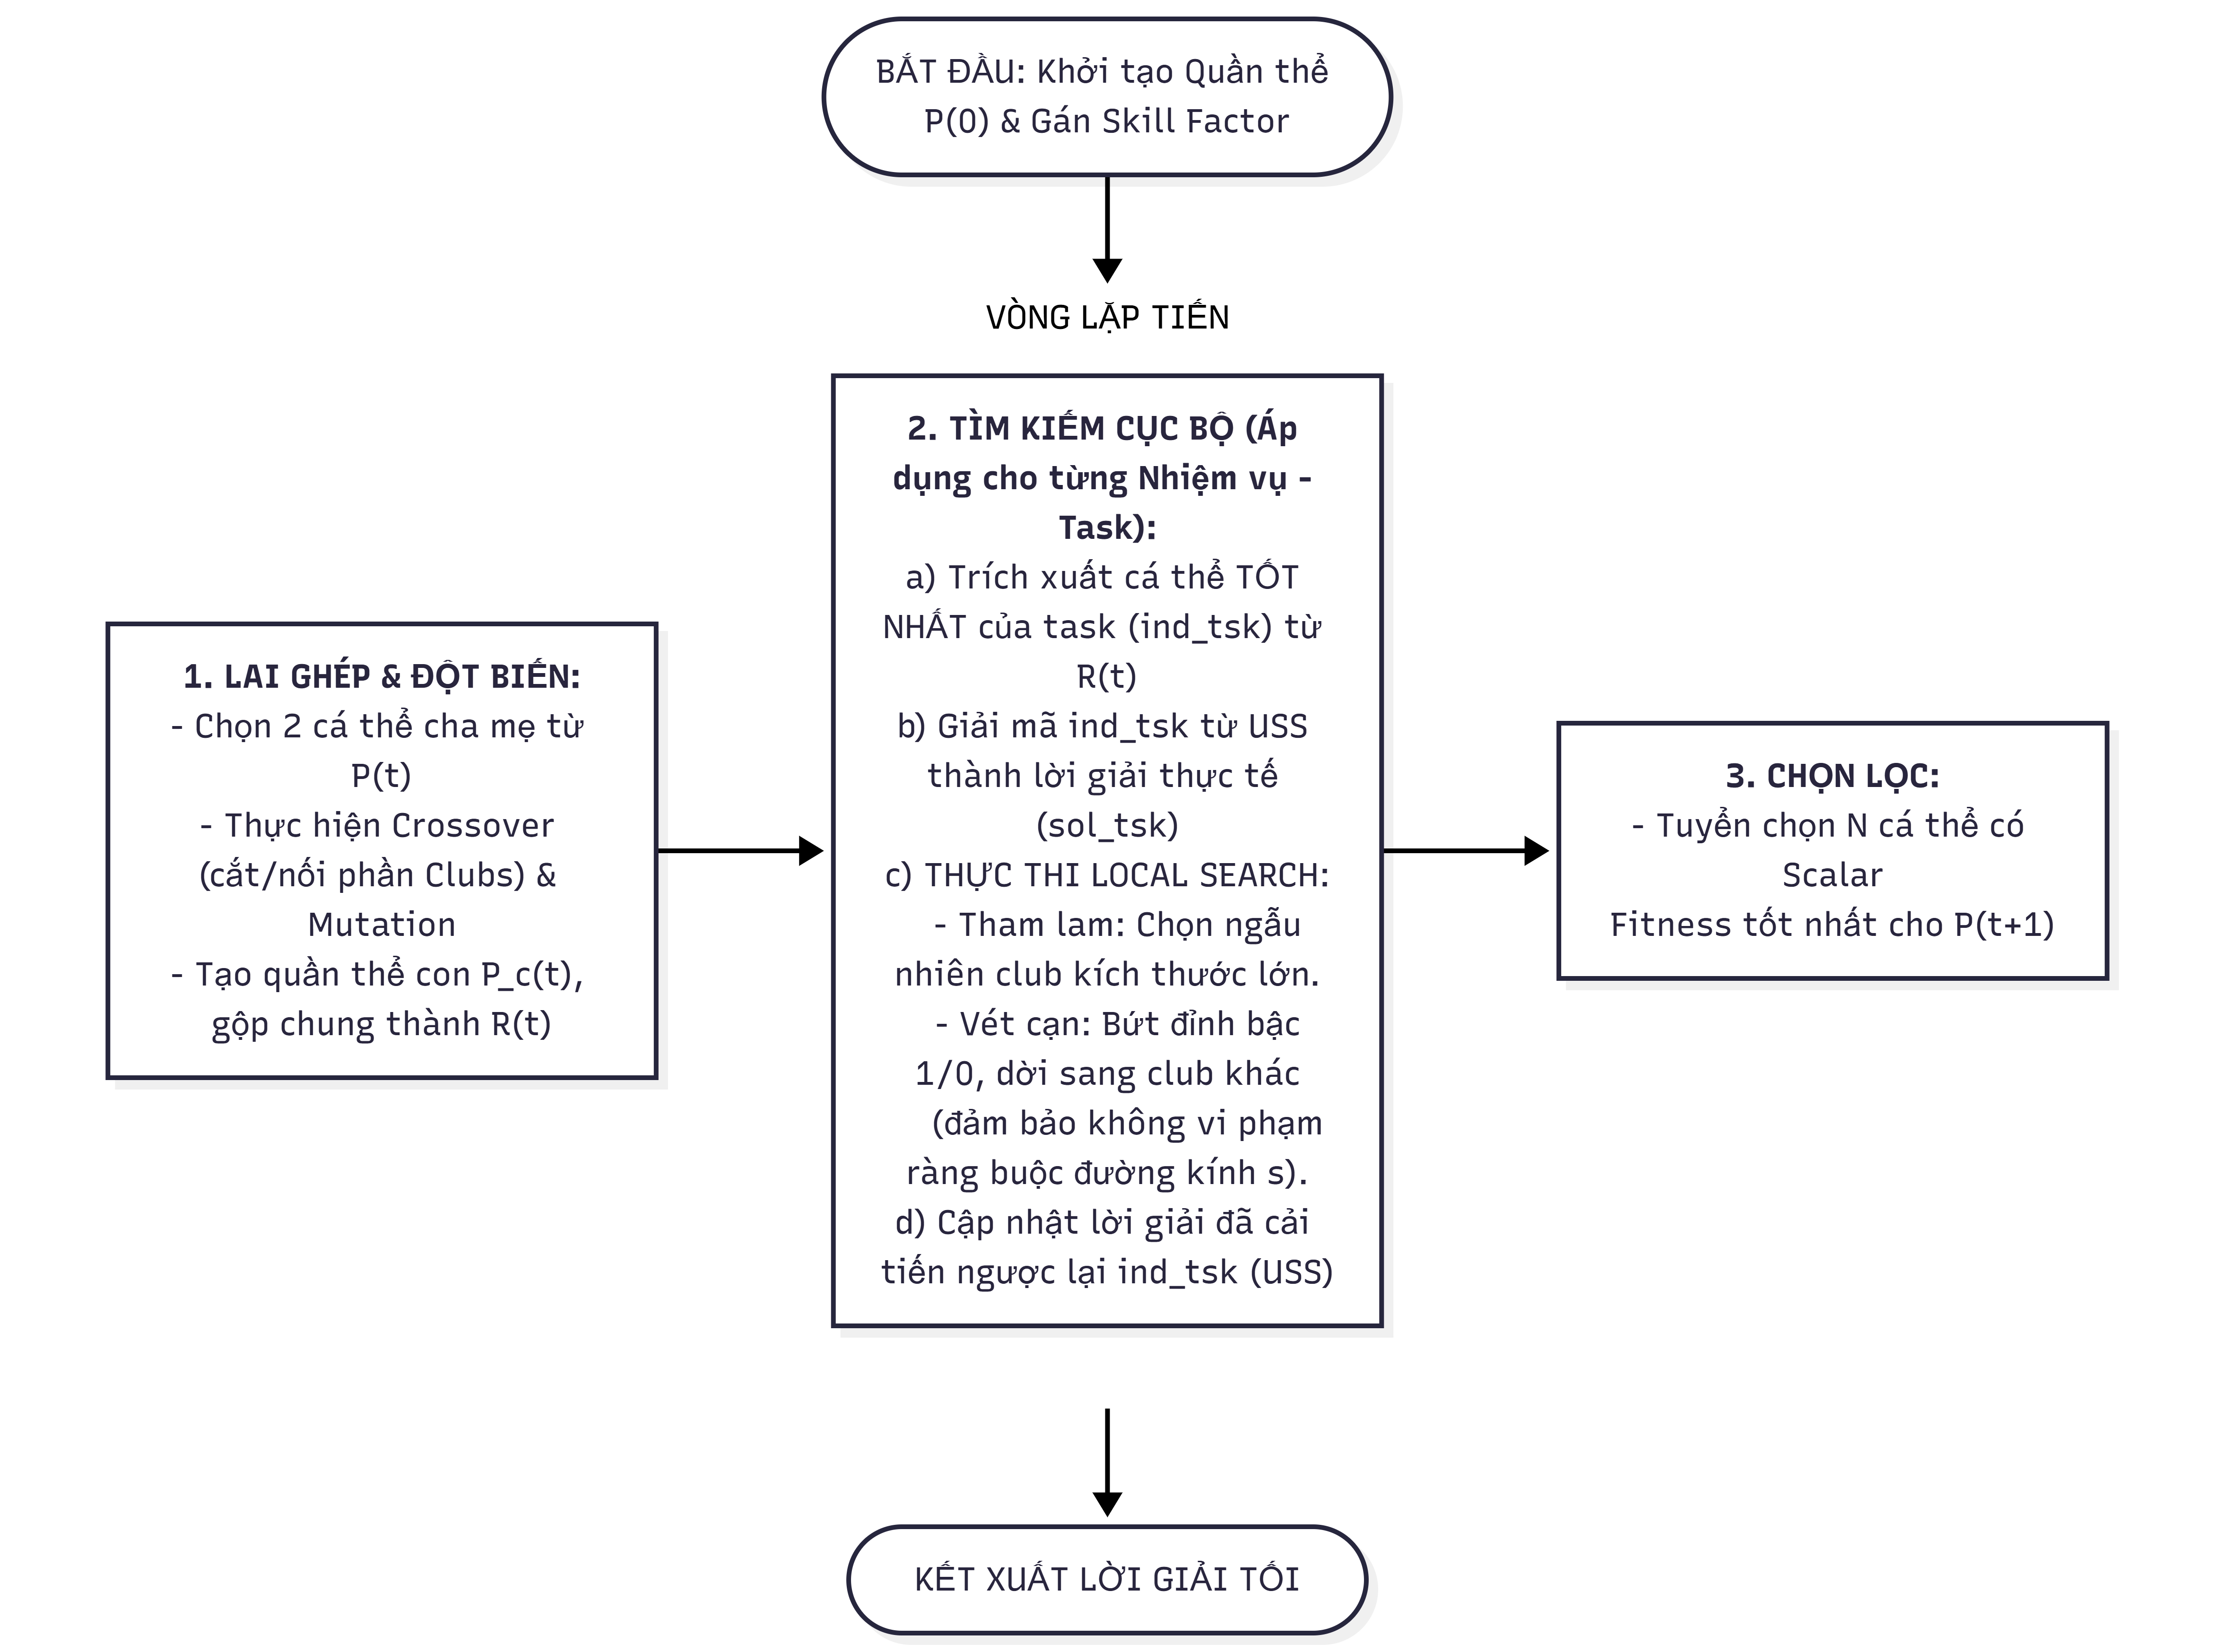
\includegraphics[width=0.9\textwidth]{Pictures/sClub_cover/sd_4_7.png}
    \caption{Sơ đồ thuật toán (Algorithm Scheme)}
    \label{fig:sClub_Definition}
\end{figure}
Thuật toán EMT-G được thiết kế nhằm giải quyết thách thức trong việc tích hợp cơ chế tìm kiếm cục bộ vào khuôn khổ tiến hóa đa nhiệm. Cách tiếp cận này được triển khai thông qua một quy trình ba giai đoạn áp dụng trên các cá thể tinh hoa. Điểm khác biệt cốt lõi của phương pháp nằm ở việc thực hiện các thao tác tối ưu trực tiếp trên cấp độ cụm (club-based), thay vì trên từng đỉnh riêng lẻ.


\begin{itemize}
    \item {Bước 1: Khởi tạo và đánh giá}
    
    Khởi tạo quần thể ban đầu $P(0)$ và tiến hành gán hệ số kỹ năng cho từng cá thể dựa trên hiệu suất của chúng trên các nhiệm vụ.
    
    \item {Bước 2: Tiến hóa (lai ghép và đột biến)}
    
    Tạo ra quần thể con thông qua việc lựa chọn ngẫu nhiên các cá thể cha mẹ, sau đó thực hiện lai ghép chéo (crossover) trên phân đoạn câu lạc bộ và áp dụng các toán tử đột biến (move, split, merge). Đối với các đỉnh chưa được phân bổ, thuật toán sử dụng chiến lược tham lam để chèn chúng vào các câu lạc bộ ưu tiên theo thứ tự kích thước tăng dần.
    
    \item {Bước 3: Trích xuất cá thể tinh hoa}
    
    Tại mỗi thế hệ, đối với từng nhiệm vụ, thuật toán lựa chọn cá thể có hiệu suất tốt nhất từ quần thể kết hợp (bao gồm cả cá thể cha và cá thể con).
    
    \item {Bước 4: Giải mã (Decoding)}
    
    Cá thể tinh hoa được giải mã từ không gian tìm kiếm hợp nhất (USS) nhằm thu được biểu diễn lời giải cụ thể tương ứng với từng nhiệm vụ, ký hiệu là $sol_{tsk}$.
    
    \item {Bước 5: Tìm kiếm cục bộ (Local Search -- tham lam và vét cạn)}
    
    Thuật toán áp dụng cơ chế tìm kiếm cục bộ lên lời giải vừa được giải mã, bao gồm các bước sau:
    \begin{itemize}
        \item Áp dụng chiến lược tham lam ngẫu nhiên (random greedy) để ưu tiên lựa chọn các câu lạc bộ có số lượng đỉnh lớn.
        
        \item Thực hiện chuyển đổi tuần tự các đỉnh từ câu lạc bộ đã chọn sang các câu lạc bộ khác. Trong đó, các đỉnh có bậc (degree) bằng $1$ (hoặc $0$) được ưu tiên xử lý, do việc loại bỏ chúng không làm vi phạm ràng buộc $s$-Club của câu lạc bộ ban đầu.
        
        \item Áp dụng chiến lược vét cạn (exhaustive strategy) để kiểm tra tính hợp lệ của câu lạc bộ đích, nhằm đảm bảo duy trì điều kiện về đường kính tối đa không vượt quá $s$.
    \end{itemize}
    
    \item {Bước 6: Cập nhật ngược và chọn lọc}
    
    Lời giải sau khi được cải thiện thông qua tìm kiếm cục bộ sẽ được ánh xạ ngược trở lại cá thể tương ứng trong không gian USS. Cuối cùng, cơ chế chọn lọc tự nhiên được áp dụng nhằm duy trì các cá thể có chất lượng tốt nhất cho thế hệ kế tiếp.
\end{itemize}



\subsubsection{Ưu điểm}
    Khác với các thuật toán tìm kiếm cục bộ truyền thống chủ yếu thao tác trên từng đỉnh (vertex-based), phương pháp này thực hiện can thiệp trực tiếp ở cấp độ tập hợp (club-based). 
    Cách tiếp cận này giúp giảm đáng kể chi phí tính toán, do hạn chế việc khám phá không gian tìm kiếm kém hiệu quả trên các đỉnh riêng lẻ không có tiềm năng cải thiện lời giải.

    EMT-G cho thấy hiệu năng vượt trội so với thuật toán di truyền cơ bản (GA), với kết quả thực nghiệm cho thấy tốt hơn trong 7 trường hợp, tương đương trong 13 trường hợp và không có trường hợp nào kém hơn. 
    Đặc biệt, phương pháp này vượt trội rõ rệt so với các thuật toán SALO và EMT-DSE khi áp dụng trên các đồ thị có mật độ lớn hơn $0.16$ và $0.09$, tương ứng.

    Cơ chế lựa chọn club dựa trên chiến lược tham lam ngẫu nhiên cho phép duy trì tính đa dạng của không gian tìm kiếm (exploration). 
    Đồng thời, kỹ thuật chuyển đỉnh dựa trên chiến lược vét cạn (exhaustive search) giúp tăng cường khả năng hội tụ nhanh tới các nghiệm chất lượng cao (exploitation). 
    Sự kết hợp này tạo nên một cơ chế cân bằng hiệu quả giữa hai quá trình khai phá và khai thác trong tối ưu hóa.

\subsubsection{Nhược điểm}
Khi so sánh với phương pháp heuristic chuyên biệt SALO, hiệu năng của EMT-G không hoàn toàn áp đảo. Cụ thể, EMT-G cho kết quả kém hơn SALO ở 3 bộ dữ liệu. Đặc biệt, trên các đồ thị có tổng số đỉnh dưới hoặc mật độ đồ thị thấp, SALO cho thấy khả năng cạnh tranh rất mạnh mẽ.

Mặc dù đã tối ưu hóa, quá trình rút và ghép đỉnh giữa các club vẫn đòi hỏi phải tính toán lại liên tục để đảm bảo không vi phạm ràng buộc giới hạn đường kính của s-Club. Chính nhóm tác giả cũng đặt ra mục tiêu trong tương lai phải làm giảm chi phí tính toán cho quá trình xác minh các club hợp lệ này.


%===----------------- subsection Covering a Graph with Clubs ----------------====
\subsection{Disjoint covering of bipartite graphs with s-clubs~\cite{monti2025disjoint}}
NGHIÊN CỨU NÀY CHƯA CHÍNH THỨC ĐƯỢC XUẤT BẢN


%===----------------- subsection Covering a Graph with Clubs ----------------====
\subsection{Exact algorithms for the minimum s-club partitioning problem~\cite{yezerska2019exact}}






%===---------------------- Results ----------------------====
\section{Kết quả và bàn luận}
\label{sec:results}
%Phần này trình bày các kết quả thu được từ nghiên cứu. Có thể sử dụng hình ảnh, bảng biểu minh họa kết quả, hỗ trợ cho phần bàn luận. Nhấn mạnh các đóng góp mới của nghiên cứu so với các nghiên cứu tương tự đã công bố.

Nếu cần thiết, có thể chia nội dung một phần của bài báo thành nhiều phần nhỏ. Khi này, có thể cung thông tin giới thiệu nội dung các phần nhỏ giữa tiêu đề của phần chính với tiêu đề của phần nhỏ đầu tiên. 

Tiêu đề các phần nhỏ (Tiêu đề cấp 2) thống nhất dùng chữ in nghiêng đậm, cỡ 11 như dưới đây.


\subsection{Chữ viết tắt}
\label{subsec:viet_tat}

Những thuật ngữ dài, được sử dụng nhiều lần có thể sử dụng chữ viết tắt. Thuật ngữ này cần được hiển thị đầy đủ ở lần đầu tiên xuất hiện trong bài viết, kèm theo ký hiệu viết tắt đặt trong ngoặc đơn. Ví dụ: "Các định hướng phát triển khoa học công nghệ (KHCN) đã đóng vai trò...".


\subsection{Các lưu ý định dạng và trình bày}
\label{subsec_Criterial}

\subsubsection{Đơn vị đo và số liệu}
Thống nhất dùng đơn vị đo theo hệ SI cho các số liệu trong bài báo. Định dạng in nghiêng cho ký hiệu các đại lượng tính toán. Số thập phân trình bày trong bài báo tiếng Việt để dấu ","; trong bài báo tiếng Anh để dấu "."


\subsubsection{Công thức toán}
Các công thức tính toán được đánh số thứ tự, đặt trong ngoặc đơn phía lề phải như minh họa bằng các công thức (1) và (2) dưới đây. Lưu ý là các ký hiệu hàm, biến được in nghiêng; ký hiệu ma trận, véc tơ được in đậm. 

\begin{equation}
	U_m(0,f) \geq u \geq \varphi + U_m(0,f)
\end{equation}
\begin{equation}
	U_m(0,f) - \alpha > c \varphi
\end{equation}

\subsubsection{Hình ảnh, bảng biểu}
Các hình ảnh (đồ thị, sơ đồ, ảnh chụp...), bảng biểu nhất thiết phải có số hiệu và tiêu đề. Số hiệu đánh theo thứ tự tăng dần của bài báo, ví dụ Hình 1, Hình 2; bảng 1, bảng 2... Số hiệu hình vẽ, bảng biểu phải được tham chiếu (giới thiệu, bình luận) trong văn bản. Khi biên tập, để phù hợp với format của trang báo, Tòa soạn có thể di chuyển vị trí của bảng biểu, hình vẽ lên đầu trang hoặc xuống cuối trang; Do đó, đề nghị tác giả không sử dụng cách giới thiệu tương tự như: "... được minh họa trong hình sau:", hay "Số liệu thống kê như trong bảng sau:". Cần tham chiếu đến số hiệu của hình, bảng, chẳng hạn như "... được minh họa trong Hình 1", hay "Số liệu thống kê như trong bảng 2".

Số liệu trong bảng phải chính xác, hình ảnh rõ nét. Độ rộng của bảng và hình vẽ bằng độ rộng của cột, hoặc của trang giấy theo khổ dọc. Nếu bảng và hình vẽ quá lớn có thể trình bày theo trang ngang (Landscape).

Cố gắng sắp xếp để hình ảnh, bảng biểu ở vị trí gần với nội dung văn bản có tham chiếu đến hình ảnh, bảng biểu.

Nếu một hình bao gồm nhiều hình nhỏ, ký hiệu các hình nhỏ bằng các chữ cái a), b), v.v... và giải thích nội dung các phần nhỏ ngay trong tiêu đề của hình.

\setlength{\intextsep}{0pt}
\renewcommand{\scalefigure}{0.8}
\noindent
\begin{figure}[h!]
	\centering
	\begin{subfigure}{.48\linewidth}
		\centering
		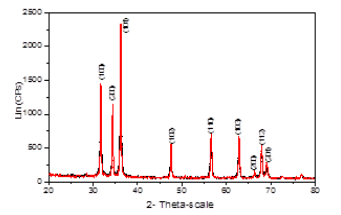
\includegraphics[scale=\scalefigure]{Pictures/pic2a.png}
		\caption{}
		\label{fig:giando_a}
	\end{subfigure}   
	\begin{subfigure}{.48\linewidth}
		\centering
		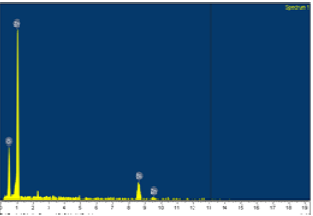
\includegraphics[scale=\scalefigure]{Pictures/pic2b.png}
		\caption{}
		\label{fig:giando_b}
	\end{subfigure}
	\caption{ (a) Giản đồ XRD của nano ZnO tổng hợp: (b) Phổ EDS của vật liệu nano ZnO }
	\label{fig:giando}
\end{figure}

Số hiệu và tiêu đề của hình để bên dưới hình. Số hiệu và tiêu đề của bảng nằm bên trên bảng. Chèn một dòng trắng vào bên trên hình và dưới tiêu đề của hình để ngăn cách với các phần văn bản phía trước và sau mỗi hình.

Hình~\ref{fig:giando} minh họa mẫu định dạng tiêu đề của một hình được chèn trong bài báo. Định dạng các thành phần của bảng biểu được minh họa như trong Bảng~\ref{tab:pt1}.

\setlength{\intextsep}{6pt}
\begin{table}[htbp]
	\centering
	\caption{Phân tích hàm lượng các nguyên tố trong lá chè (mg/kg)}
	\begin{tabular}{crrrrrrr}
		&       &       &       &       &       &       &  \\
		\midrule
		\textbf{Mẫu} & 
		\textbf{Mn} & 
		\textbf{Al} & 
		\textbf{Fe} & 
		\textbf{Zn} & 
		\textbf{Cu} & 
		\textbf{Ba} & 
		\textbf{Sr} \\
		\midrule
		MC1 & 741.92 & 260.22 & 61.88 & 31.85 & 13.64 & 13.04 & 14.95 \\
		MC2 & 1179.39 & 282.44 & 85.14 & 33.58 & 16.39 & 4.36  & 7.19 \\
		MC3 & 1239.37 & 273.67 & 86.6  & 34.69 & 15.23 & 11.97 & 8.4 \\
		MC4 & 923.03 & 281.94 & 81.48 & 31.28 & 15.58 & 6.1 & 7.61 \\
		MC5 & 918.55 & 201.7 & 67.41 & 39.79 & 14.62 & 7.04 & 9.14 \\
		MC6 & 613.33 & 189.2 & 65.76 & 27.67 & 14.55 & 12.12 & 10.56 \\
		\textbf{Trung bình} & \textbf{762.25} & \textbf{324} & \textbf{74.95} & \textbf{30.33} & \textbf{14.38} & \textbf{15.02} & \textbf{11.92} \\
	\end{tabular}%
	\label{tab:pt1}%
\end{table}%

\textbf{Lưu ý:} Các thành phần của bảng biểu phải ở dạng văn bản chỉnh sửa được, không để dưới dạng ảnh chụp màn hình. 




%===--------------------- Conclusion ---------------------====
\section{Kết luận}
\label{sec:conclusion}
%Phần này tóm tắt những kết luận quan trọng rút ra được từ phần Kết quả và Bàn luận. Lưu ý tránh trùng lặp nội dung với phần Tóm tắt. Có thể trình bày các định hướng nghiên cứu, phát triển, ứng dụng kết quả nghiên cứu.
%

%===------------------- Acknowledgements -----------------====
\section*{Lời cám ơn} 
\label{Acknowledgment}
%Gửi lời cám ơn các cá nhân, tổ chức đã đóng góp, tài trợ cho nghiên cứu. Phần này có tính tùy chọn.	

%===------------------- Acknowledgements -----------------====
%\section*{Tài liệu tham khảo} 
%\label{References}
%Danh mục tài liệu tham khảo chỉ liệt kê những tài liệu được trích dẫn trong bài báo. Ngược lại, tài liệu nào được tham chiếu trong bài cũng phải liệt lê trong danh sách tài liệu tham khảo. Yêu cầu thực hiện trích dẫn theo định dạng IEEE. Tác giả nên sử dụng các phần mềm quản lý tài liệu tham khảo chuyên dụng (như Endnote; Zotero; Biblioscape;...), hoặc sử dụng chức năng Insert Citation trong Microsoft Word để tự động hóa việc trích dẫn và định dạng danh mục tài liệu tham khảo một cách tự động, chính xác theo đúng chuẩn quốc tế.

Một số lưu ý quan trọng như sau:

Trong bài báo, tham chiếu đấn tài liệu trích dẫn bằng cách sử dụng dấu []. Dấu này cần được đặt trước dấu ngắt câu. Ví dụ: \cite{lima_node-depth_2016}, \cite{lima_node-depth_2016, perfecto_simulation-based_2016, wu_clustered_2014} hoặc [1, 3]. Khi cần tham chiếu đến số trang của tài liệu, sử dụng ký hiệu p. hoặc pp., theo sau là số trang; ví dụ [5] (p. 10). or [6] (pp. 101–105). 
Tài liệu tham khảo để cuối bài viết, chỉ sử dụng tiếng Anh. Lưu ý là các tạp chí trong nước xuất bản bằng tiếng Việt đều có tên bài báo và tóm tắt bằng tiếng Anh. Tác giả cần sử dụng những thông tin nguyên gốc này để đảm bảo người đọc có thể truy tìm tài liệu tham khảo khi cần. Những tài liệu không có thông tin bằng tiếng Anh cần dịch sang tiếng Anh và ghi chú rõ (Ví dụ: In Vietnamese). 

	



%===------------------ Tai lieu tham khao ----------------====
\setlength{\bibsep}{3pt}
\fontsize{11}{11}\selectfont
\bibliographystyle{ieeetr}
\bibliography{references}



\end{document}